\documentclass[11pt,letterpaper]{article}
\usepackage[margin=0.6in]{geometry}
\usepackage{amsmath,amssymb}
\usepackage{tikz}
\usetikzlibrary{arrows.meta,positioning,matrix}
\usepackage{xcolor}
\usepackage{fontawesome5}
\usepackage{tcolorbox}
\usepackage{multicol}
\usepackage{enumitem}
\usepackage{hyperref}

\definecolor{primaryblue}{RGB}{41, 98, 255}
\definecolor{accentgreen}{RGB}{0, 150, 136}
\definecolor{warnorange}{RGB}{255, 152, 0}
\definecolor{lightgray}{RGB}{245, 245, 245}

\tcbset{
    conceptbox/.style={colback=primaryblue!5, colframe=primaryblue, boxrule=1pt, arc=3pt, left=5pt, right=5pt, top=5pt, bottom=5pt},
    formulabox/.style={colback=lightgray, colframe=gray!50, boxrule=0.5pt, arc=2pt, left=5pt, right=5pt, top=3pt, bottom=3pt},
    warningbox/.style={colback=warnorange!10, colframe=warnorange, boxrule=1pt, arc=3pt, left=5pt, right=5pt, top=5pt, bottom=5pt},
    appbox/.style={colback=accentgreen!5, colframe=accentgreen, boxrule=1pt, arc=3pt, left=5pt, right=5pt, top=5pt, bottom=5pt}
}

\pagestyle{empty}
\setlength{\parindent}{0pt}
\setlist[itemize]{leftmargin=*, itemsep=1pt, topsep=2pt}

\begin{document}

\begin{center}
{\LARGE\bfseries\color{primaryblue} Chapter 6: Matrix Decomposition}\\[3pt]
{\large SVD, Eigendecomposition, and PCA}
\end{center}
\vspace{-5pt}
\hrule height 2pt
\vspace{8pt}

\begin{multicols}{2}

\begin{tcolorbox}[conceptbox, title={\faLightbulb\ Key Concepts}]
\begin{itemize}
    \item \textbf{SVD}: Any matrix = $U\Sigma V^T$
    \item \textbf{Eigendecomposition}: Square matrix = $Q\Lambda Q^{-1}$
    \item \textbf{Singular Values}: ``Importance'' of each component
    \item \textbf{Low-Rank Approximation}: Keep top-$k$ components
    \item \textbf{PCA}: Find directions of maximum variance
\end{itemize}
\end{tcolorbox}

\begin{tcolorbox}[formulabox, title={\faCalculator\ Core Formulas}]
\textbf{SVD:}
\[ A = U \Sigma V^T \]
$U$: left singular vectors, $\Sigma$: singular values, $V$: right singular vectors

\textbf{Low-Rank Approximation:}
\[ A_k = \sum_{i=1}^{k} \sigma_i \mathbf{u}_i \mathbf{v}_i^T \]

\textbf{Eckart-Young Theorem:}
\[ A_k = \arg\min_{\text{rank}(B)=k} \|A - B\|_F \]

\textbf{PCA via SVD:}
\[ X = U\Sigma V^T \Rightarrow \text{PCs} = V \]
\end{tcolorbox}

\columnbreak

\begin{center}
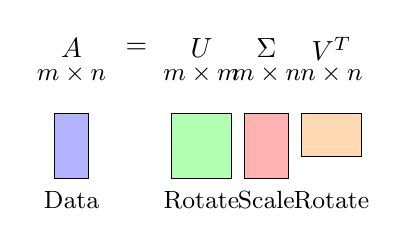
\begin{tikzpicture}[scale=0.55]
    % SVD visualization
    \node at (0,0) {$A$};
    \node at (0,-0.6) {\small $m \times n$};

    \node at (1.5,0) {$=$};

    \node at (3,0) {$U$};
    \node at (3,-0.6) {\small $m \times m$};

    \node at (4.5,0) {$\Sigma$};
    \node at (4.5,-0.6) {\small $m \times n$};

    \node at (6,0) {$V^T$};
    \node at (6,-0.6) {\small $n \times n$};

    % Visual representation
    \draw[fill=blue!30] (-0.4,-1.5) rectangle (0.4,-3);
    \draw[fill=green!30] (2.3,-1.5) rectangle (3.7,-3);
    \draw[fill=red!30] (4,-1.5) rectangle (5,-3);
    \draw[fill=orange!30] (5.3,-1.5) rectangle (6.7,-2.5);

    \node at (0,-3.5) {\small Data};
    \node at (3,-3.5) {\small Rotate};
    \node at (4.5,-3.5) {\small Scale};
    \node at (6,-3.5) {\small Rotate};
\end{tikzpicture}
\end{center}

\begin{tcolorbox}[appbox, title={\faRobot\ ML Applications}]
\begin{itemize}
    \item \textbf{PCA}: Dimensionality reduction, visualization
    \item \textbf{Image Compression}: Keep top-$k$ singular values
    \item \textbf{Recommender Systems}: Matrix factorization
    \item \textbf{Latent Semantic Analysis}: Topic modeling
    \item \textbf{Model Compression}: Low-rank weight approximation
\end{itemize}
\end{tcolorbox}

\begin{tcolorbox}[warningbox, title={\faExclamationTriangle\ Common Pitfalls}]
\begin{itemize}
    \item \textbf{Center data} before PCA (subtract mean)
    \item SVD of $X$ $\neq$ eigendecomposition of $X$
    \item Singular values are always $\geq 0$, eigenvalues can be negative
    \item Truncated SVD loses information --- check reconstruction error
\end{itemize}
\end{tcolorbox}

\end{multicols}

\vspace{5pt}
\hrule
\vspace{5pt}

\begin{center}
\faGithub\ \textbf{Notebook}: \url{https://github.com/vijaygwu/math-powers-ai/blob/main/notebooks/ch06_svd_compression.ipynb}
\end{center}

\end{document}
